\documentclass[a4paper]{article}
 \usepackage{fullpage}
\usepackage{amsfonts} % pour les lettres maths creuses \mathbb
\usepackage{amsmath}
\usepackage[T1]{fontenc}
\usepackage[utf8]{inputenc}
\usepackage[frenchb]{babel}
\usepackage{aeguill}
\usepackage{graphicx}
\usepackage{hyperref}
\usepackage{color}
\usepackage{listings}
\usepackage{pdfpages}

\newcommand\dx{\dot{x}}
\newcommand\dy{\dot{y}}
\newcommand\ddx{\ddot{x}}
\newcommand\ddy{\ddot{y}}
\def\real{{\mathbb R}}
\frenchbsetup%
{%
StandardItemLabels=true,%
ItemLabels=\ding{43},%
}%

\author {}
\title {Cover letter for the IJRR submission \\ ``An efficient acyclic contact planner for multiped robots''}
\date {}
\begin{document}
\maketitle

Dear Editor, \\
first of all we thank you for the time spent on considering our orignal manuscript. Indeed,
%This cover letter for the manuscript ``An efficient acyclic contact planner for legged robots'' plays more the role of a rebutal, since the paper is a resubmission for the ISSR'15 sepcial issue, and that we ask for reviewer continuity.
this cover letter introduces the first revision of the manuscript ``An efficient acyclic contact planner for legged robots'', resubmitted for the ISSR'15 sepcial issue.
As discussed with prof. Hollerbach, we hoped to have reviewer continuity for the revision.
The cover letter then plays more the role of a rebutal. We left the original cover letter at the end of this document, as well as the original ISRR reviews.
Therefore, we kindly ask that this cover letter be forwarded to the reviewers of the new manuscript.

We would then like to thank the reviewers for their previous feedback on the initial manuscript. We believe we have answered
all of their concerns, the main ones being that our method had not been tested on a real robot or a simulation, and that the paper was too verbose.
In the following lines we are going to describe how we improved our paper in this regard, and answer to the other remarks of the reviewers.

\section{Recall of main paper contributions}
The paper is concerned with the problem of planning acyclic contact planning. 
More precisely, we propose a very efficient method to address what we believe is the core of the difficulty of the contact planning problem: discovering the sequence of key contact postures that would lead to a safe and stable contact trajectory of the robot. 
Using the terminology of the paper, our contact planner addressed the two sub-problems $\mathcal{P}_1$ (finding a guide path for the robot root) and $\mathcal{P}_2$ (finding a sequence of stable contact postures and corresponding contact locations).
Our claim is that the solution of our planner leads to a straight-forward resolution of the last sub-problem $\mathcal{P}_3$ (finding the complete trajectory connecting the contact postures).
In particular, our method proposes interactive performances, i.e. the planner needs less time to compute the solution than what is needed for the robot to execute it.
This practical result corresponds to a significant improvement of the state of the art, for example regarding the capabilities of acyclic contact planners demonstrated by the humanoid teams during the Darpa Robotics Challenge last year.

Regarding this contribution, the reviews mostly criticized the structure of the paper (too verbose) and the unjustified claim that the contact sequence output by the planner leads to a feasible resolution of $\mathcal{P}_3$.

In the revision, we implemented a solver inspired by the state of the art to solve $\mathcal{P}_3$ and empiricially proved the claim that our $\mathcal{P}_1$-$\mathcal{P}_2$ planner leads to easily solving $\mathcal{P}_3$. 
All the robot contact sequences reported in the paper have been converted to full contact trajectories using this $\mathcal{P}_3$ solution.
We also executed one of them on the real robot.
This extension, along with the correction of the other remarks by the reviewers, have been integregated in the revision paper, that we also reworked to make it clearer, shorter and sharper (the core of the paper is now 13 pages long, as opposed to 17 before) than the original manuscript.

The details of these modifications follow.

\section{Validation of the method (addressing  $\mathcal{P}_3$) }
In his review, reviewer 2 stated that our plans are likely to be not executable, even in simulation.

\begin{quote}
  \textit{A quick glance at the sequences displayed in the video reveals that the "motion patterns" (and I understand these are not "motions" per se, but "contact plans") are not physically consistent (even reagrding them as mere contact plans and not as the final motions). The robot moves a contact without needing to readjust the posture in order to release that contact (or "set it free", by nullifying the contact forces on that contact). This results in sequences in which the contacts seem to be "slided" rather than removed and repositioned. This denotes a significant flaw in the algorithm.   }
\end{quote}

We were really surprised by the remark, in particular because we had already validated some of our plans.
The stair climbing scenario has been demonstrated on the real HRP-2 robot, while the standing up had been demonstrated in simulation. 
While it was mentioned in the paper, we did not insist on these demonstrations because our main contribution focuses on the other problems. 
We believe that, as reviewer 1 notices, this observation was due to the fact that we did not clearly define what we mean by a contact plan (i.e. a discrete sequence of key contact posture with the corresponding contact locations).
We thank the reviewers for these comments, since it pointed out that what we believed to be an evidence must be carefully explained and justified.

A rigorous definition of a contact plan is now detailed in section 5.1. 

%In any case, the validation videos joined to the submission should now establish that our plans are in indeed feasible, even without considering the torque constraints.

We also implemented a solver inspired by the state of the art to dynamically interpolate the contact plan and produce a complete trajectory of the robot, that we validated in a full-dynamics simulator. 
This implementation completely validates that the contact plan is feasible by the real robot.
We also indeed executed one of the computed trajectory (climbing the stairs with HRP-2).

We have joined the full-dynamics simulation and real life videos of all the scenarios we demonstrate.
These videos show that the plans we compute correspond to feasible motions.
While we briefly describe how we solve $\mathcal{P}_3$, the focus of the paper remains $\mathcal{P}_1$ and $\mathcal{P}_2$. 
The solution of $\mathcal{P}_3$ is reported in the appendix to emphasize the main focus.

\newcommand{\mP}[1]{$\mathcal{P}_#1$}

\section{Success rates of the method}
At this point, we believe it is important to clarify our position regarding the concerns of both reviewers about the success rates of our paper.
In the paper, we are providing the success rates of our contact planner. 
Such an empirical study has yet never been provided for other contact planners.
Our method is not always successful, as very often with probabilistic searches.
More precisely, the hypothesis taken by \mP1 may lead to an infeasible \mP2 problem, and similarly \mP2 hypotheses may lead to an infeasible \mP3.
We accept this fact and argue that it is mostly successful (i.e. more than 77\% of success in reasonable ``DRC-like'' scenarios).
Even in case of failure, the planner is based on random sampling that approximate probabilistic completeness, and can be restarted to obtain another candidate trajectory.
In practice, it can always find a feasible solution fast enough for online applications by replanning upon failure.

In previous works, it is in fact unknown whether the methods are always successful or not. We simply have no idea. For instance, the CIO of Mordatch,
because of the local convergence of the method, \textbf{necessarily} fails in some scenarios. We just do not know how often. Similarly, Escande et al. had to manually edit 
the end effector trajectories to avoid collisions with the environment, but we do not know how often. Considering this,
we do not understand why we are criticized for providing our success rates, which actually demonstrate the interest of our approach.

\section{Originality and interest of the work}
We strongly disagree with reviewer 2 regarding the originality of the work when he states that we simply ``\textit{experiment with minor heuristic adjustments}''.
Bretl formalized well the problem without providing an algorithm applicable to the general case. Escande focused on the contact planning $\mathcal{P}_2$. 
Our work tackles $\mathcal{P}_1$ as well, in a much more efficient manner than Bouyarmane et al.. 
These works, including the one of Hauser, are limited by the computational complexity of considering the full dimension of the problem.


The reachability condition provides a dimensionality reduction of the problem. This is clearly an originality regarding the previous work who always consider the whole-body problem.
We believe that this reduction is the only way to make the contact planning problem tractable, in the same way that many researchers (such as ourselves, but also Wieber, Tedrake, Righetti and others) use dimensionality reduction successfully to address
the trajectory optimization problem $\mathcal{P}_3$.

Furthermore, the computational time provided by our method is a contribution in itself: it makes the difference
between a method that can be used at the Darpa challenge or not, as we show in our introduction.

\section{A clearer paper}
As requested, we have deeply shortened the paper. More importantly, we have done an important work of defining in simpler terms
the different concepts that we use in the paper, and reduced their number.
We believe that the paper is much more clearer in its current form.

\section{Justification of the simplifying assumptions}
Regarding several comments from both reviewers, stating that our paper does not justify the fact that contact feasibility implies equilibrium feasibility,
we now have added a section that discusses in depth the assumption (Section 7). We clearly describe which hypothesis (we call it the quasi-flat hypothesis, referring
to the contacts in the configurations, rather than the vague cluttered term) are required to validate our approach, and analyze
the success rates we obtained in each scenario to justify that the assumption works.

\section{Comparison with other methods}
As noted by reviewer 2, in our previous paper it was indeed complex to compare our work with previous contributions,
since they were adressing the complete problem. We now give the complete computation times and compare them with previous works,
clearly demonstrating that our method outperforms them by orders of magnitude (Section 6.4).


\section{On the static equilibrium of each configuration}
Reviewer 1 stated that ``\textit{the planned contact path is only discrete with static equilibrium considered for each
configuration, which is not very realistic''}. While we agree with the observation, we first recall that this assumption is made in the previous works that address cluttered scenarios, such as the work from Bretl and Escande. Works that do not make this assumption such as Mordatch and al. only offer local convergence and can't address these scenarios. Furthermore, this limitation is in fact less restrictive in our approach that the one of Escande, since while our plan is quasi static, our resulting motion is dynamic, as now explained in the paper (Section 5.1). 

\section{Actual car model of the DARPA Challenge}
As asked by reviewer 2, we now use the polaris car model for demonstrating our egress scenario.

\end{document}


\author {}
\title {Original Cover letter for the IJRR submission \\ ``An efficient acyclic contact planner for multiped robots''}
\date {}
\begin{document}
\maketitle

Dear editor and reviewers, \\ \\

The current submission is an extension to our conference paper ``A reachability-based planner for sequences of acyclic contacts in
cluttered environments'', accepted to ISRR 15 (\url{http://stevetonneau.fr/files/publications/isrr15/isrr15.pdf}).

In these two papers, our objective is to propose automatic methods
to compute the contact sequence that characterizes a robot motion in
cluttered environment.

We joined to the present submission the reviews that were made on the
conference paper. They follow the cover letter.

Regarding the conference paper, this apper paper presents new contributions that we first highlight:

\begin{itemize}
\item We introduce a new criterion for asserting the static equilibrium of a robot configuration. It works for arbitrary
legged robots, and handles any kind of contact configurations and surface orientation. It is formulated as a really efficient Linear Program, and 
can be used to compute a value of robustness of the configuration. This robustness is useful for real robots applications, where many uncertainties
in the state estimation of the robot can lead to incorrect evaluations of the equilibrium.
\item We present two new heuristics that we use to bias our contact planner framework towards configurations relevant for the task being performed.
\item We present a complete algorithm for contact planning that integrates the robust equilibrium criterion.
\end{itemize}

The extension of our work also addresses the main comments of the reviewers, and proposes lesser contributions,
that we detail in the following lines.

\begin{itemize}
\item They were concerned by the fact that our demonstrations were
considering virtual avatars and not actual robots. In the present
submission, all our examples are applied to the HRP-2 and HyQ robots (Section 6).
To achieve this, a new contribution is proposed in our paper:
We introduce a robustness criterion for asserting the static equilibrium
of a configuration (Section 5.1). We use it in combination with new heuristics that we
propose to bias the contact generation process towards configurations
relevant for the motion being performed (Section 5.2).
With the exception of the dextrous hand, all the demonstrations shown in
the paper and the video are entirely new.

\item They also judged that the conference paper provided a theoretical
description of our approach, but lacked the details on how to apply
the method on an actual robot. We now explain the complete process
for the HRP-2 in the present submission (Appendix A).

\item Concerning remarks made on the reproducibility of the method,
we now provide the complete pseudo code of the algorithm, as well as the
source code of our application (Appendix B).

\item The paper has been largely re-written: we provide a clearer
comparison to the state of the art (Section 1.1); we clarify our statement regarding
our computation times and compare our method with the state of the art (Section 6); we make a clear distinction between the
theoretical concepts we propose and their approximation (Section 2).

\item Regarding the computation time performances, compared to our conference paper, the planner is much more efficient.
A fundamental change is the reimplementation of the algorithm as a Bi-RRT planner instead of the PRM
approach. The code is also more efficient thanks to its complete rewriting into the HPP platform.

\item Finally, we propose an analysis of the performances of our method and
the success rates we obtained for each scenario (Section 6.2). This analysis provides
a support for our argumentation on the strong choices made in the design
of our planner (Section 1.2 and 2), and a comparison with methods from the literature.
\end{itemize}

We are convinced that these points not only provide a complete answer to
the reviews of the conference paper, but also bring new contributions to
the community, that justify a journal publication.

%~ On a last note, as required by the IJRR submission form,
%~ we proposed a list of editors and reviewers for the submission.
%~ We affirm that we don't have conflicts of interest with the people we propose.
%~ For complete clarity however, we want to mention that some of the authors
%~ are proposing two workshops for the ICRA conference this year.
%~ Among the names we proposed for reviews, Karen Liu, kris Hauser, and Quang-Cuong Pham have accepted to be invited speakers.

We thank the editor and the reviewers for their time.


Sincerely, \\

The authors

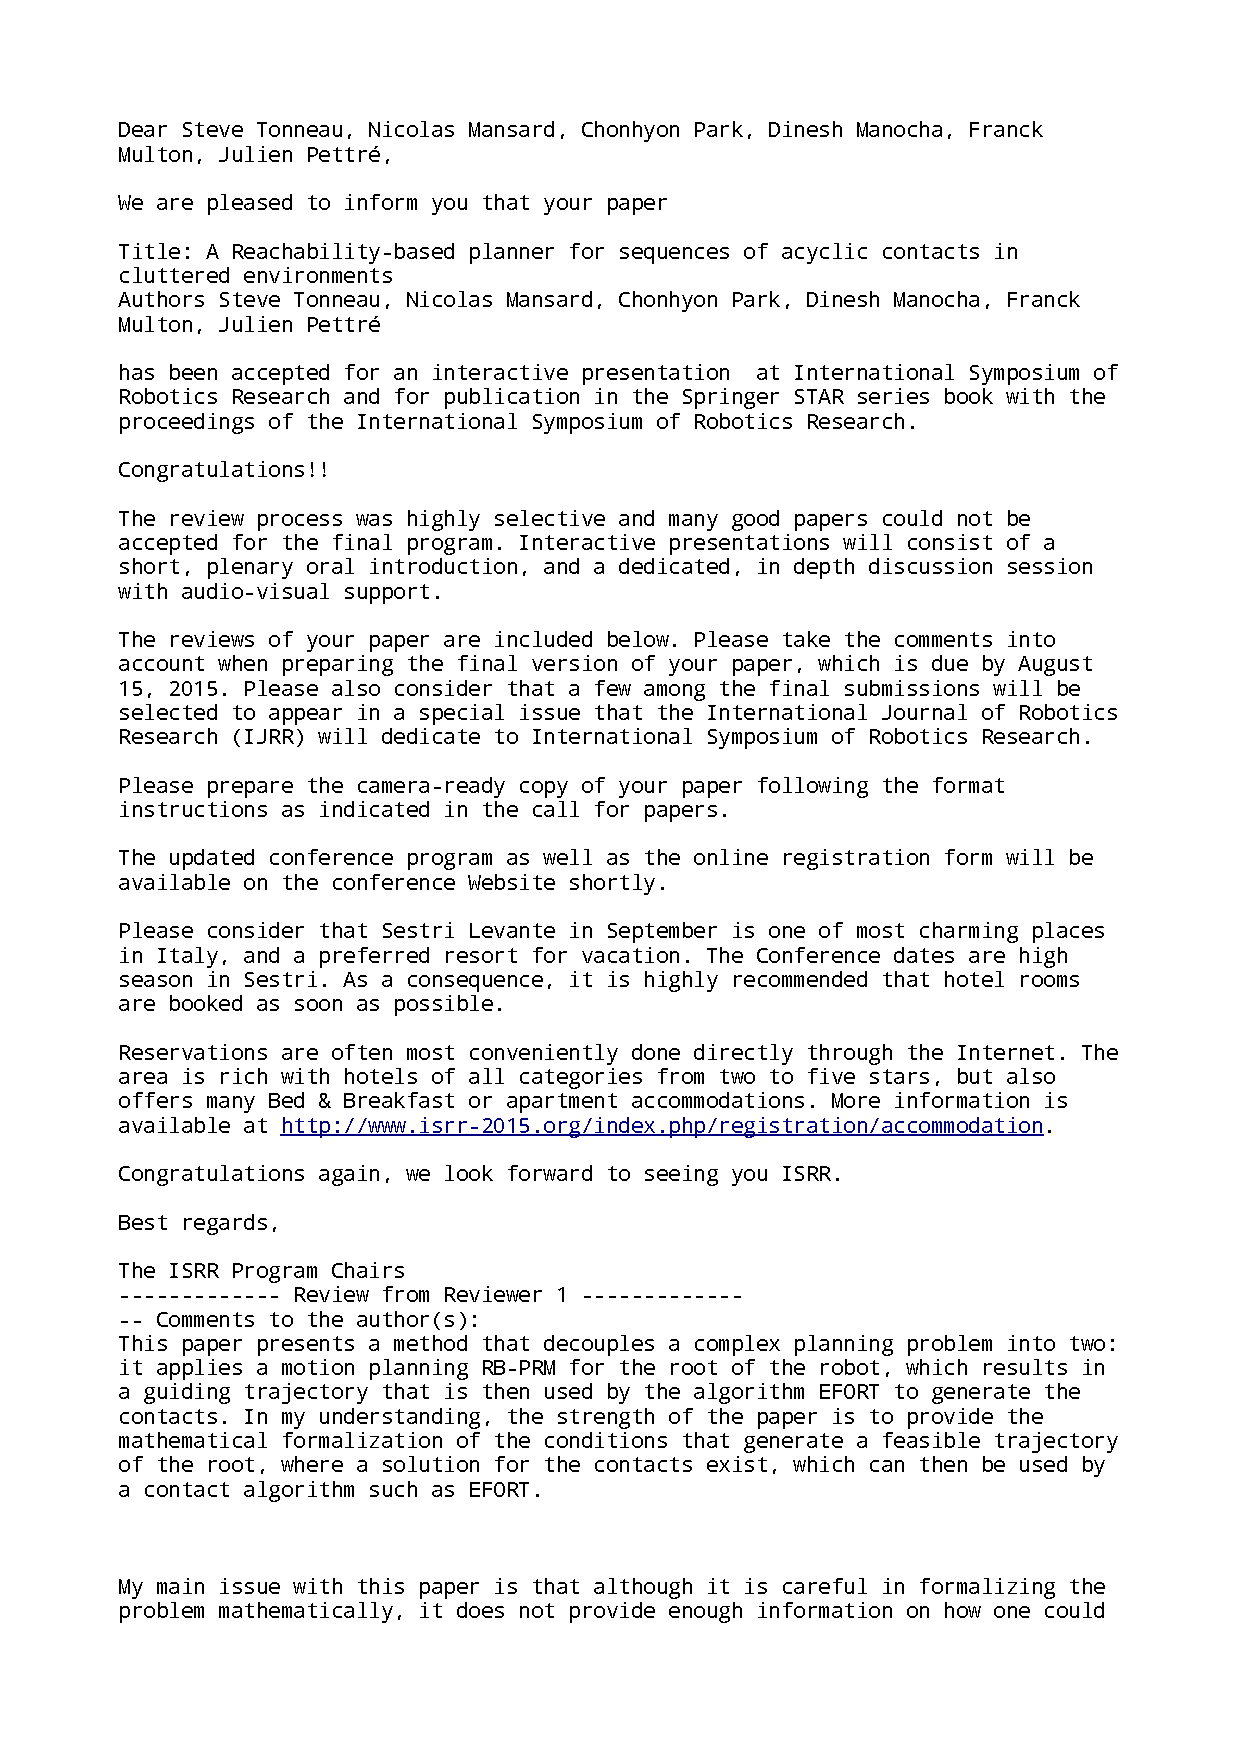
\includepdf[pages=-]{reviewisrr.pdf}


\end{document}
